\documentclass{article} \usepackage{graphicx} \usepackage[utf8]{inputenc} \author{C and bash} \title{Równiania} \begin{document} \maketitle
\section{1.0x^2+20.0*x+1.0} Mamy funkcje 1.0x^2 + 20.0x + 1.0 \Delta = 20.0^2 - 4\times1.0\times1.0 x_1 = \frac{-20.0 + \sqrt{396.0}}{2\times1.0} x_2 = \frac{-20.0 - \sqrt{396.0}}{2\times1.0} x_1 = 0.0 x_2 = 0.0 \newline \begin{tabular}{|c|c|} \hline 1.0 & 22.0 \\ 2.0 & 45.0 \\ \hline \end{tabular} \end{1.0x^2+20.0*x+1.0}
\\\
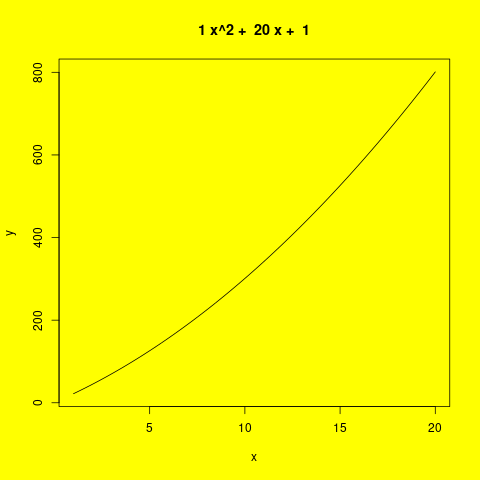
\includegraphics[width=\linewidth]{charts_tmp/0img.png}
\section{20.0x^2+420.0*x+1.0} Mamy funkcje 20.0x^2 + 420.0x + 1.0 \Delta = 420.0^2 - 4\times20.0\times1.0 x_1 = \frac{-420.0 + \sqrt{176320.0}}{2\times20.0} x_2 = \frac{-420.0 - \sqrt{176320.0}}{2\times20.0} x_1 = 0.0 x_2 = 0.0 \newline \begin{tabular}{|c|c|} \hline -41.0 & 16401.0 \\ -40.0 & 15201.0 \\ \hline \end{tabular} \end{20.0x^2+420.0*x+1.0}
\\\
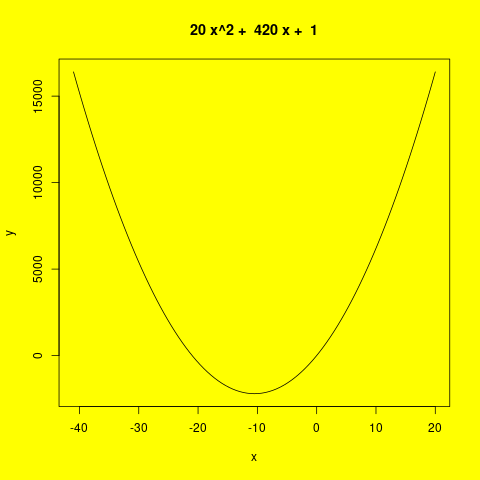
\includegraphics[width=\linewidth]{charts_tmp/1img.png}
\end{document} \end{article}
